% !TEX root = ../PhD Thesis.tex
\chapter{psichomics}

\begin{figure}[!b]
  \vspace*{-.5cm}
  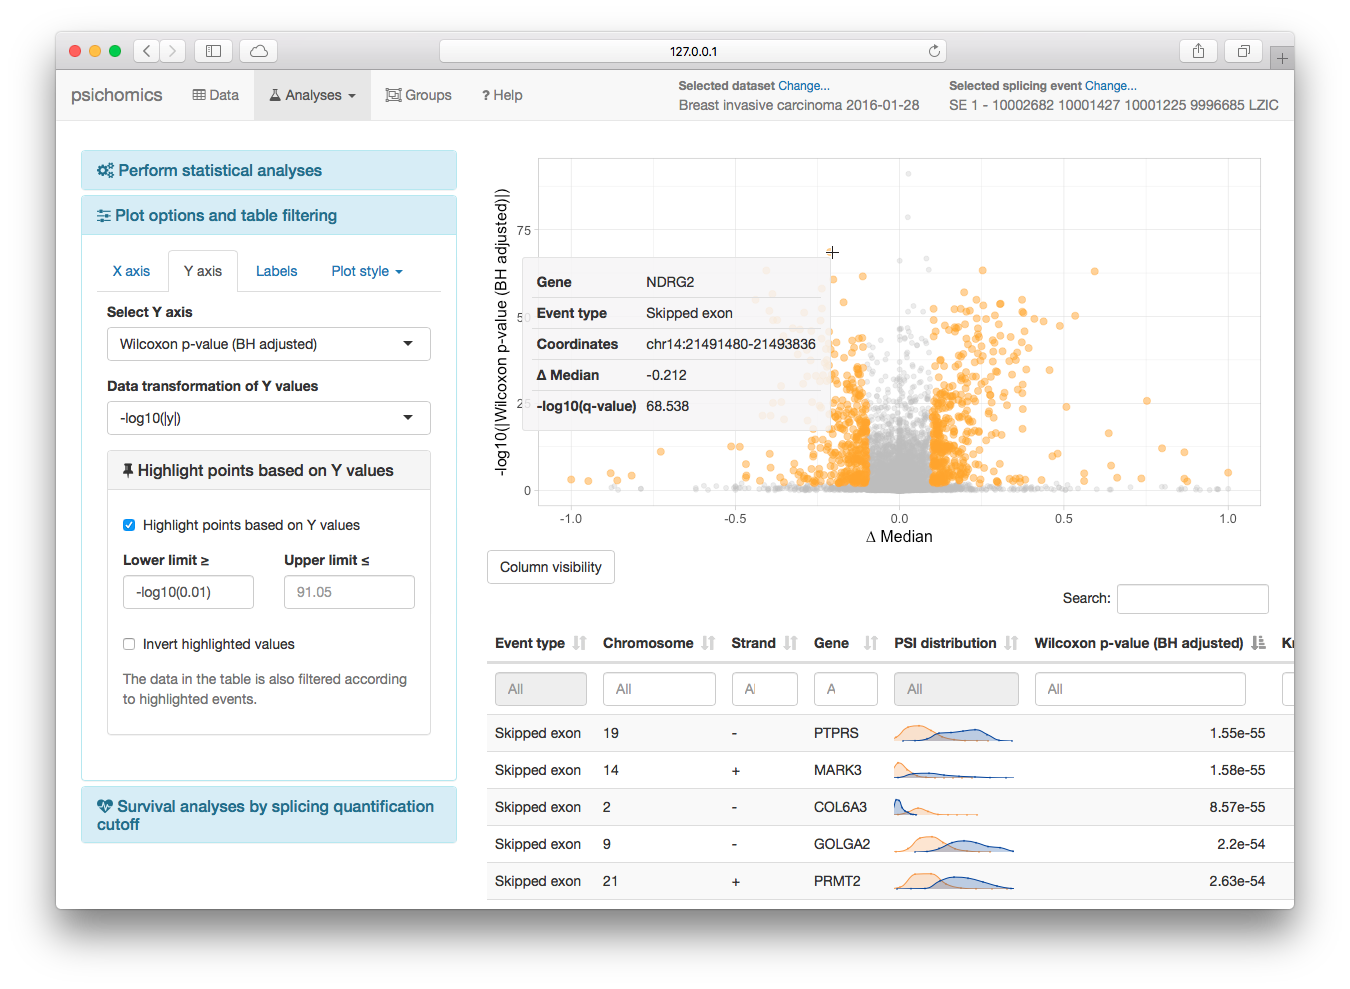
\includegraphics[width=.93\textwidth]{images/psichomics/screenshot}
  \centering
  \vspace*{-.5cm}
  \caption[psichomics screenshot]{\textbf{psichomics screenshot.} TCGA breast cancer splicing analysis (28 Jan 2020).}
  \label{fig:psichomics-screenshot}
\end{figure}

After finishing the first year of my Masters in Informatics, I was looking for a challenging thesis where I could apply all that I learned into a bioinformatics project. While looking for computational biology groups, I found out about Nuno Morais lab, a research group interested in studying transcriptomics in disease.

Nuno made me aware of the need for graphical, interactive tools to allow non-experts to analyse and visualise splicing from processed big datasets. I loved the idea and started exploring ways of going from concept to reality. After toying with multiple frameworks and programming languages, I decided to stick with the R statistical language and the Shiny web app framework \cite{chang:2021ul} that helped me to kick-start what would be later known as psichomics (\shortref{fig:psichomics-screenshot}).

psichomics was first made available in 2016 via Bioconductor to quantify, analyse and visualise alternative splicing using TCGA data \cite{chang:2013ww}. Later on, I started my PhD project in the same lab and continued my work on psichomics. Nowadays, the tool allows to analyse gene expression and alternative splicing based on user-provided or public transcriptomic data, including those from TCGA \cite{chang:2013ww}, GTEx \cite{lonsdale:2013uo} and recount2 \cite{collado-torres:2017uw} (\shortref{tab:psichomics}).

% Following an invitation from Springer Methods, I also prepared a book chapter on using psichomics to analyse alternative splicing in stem cell differentiation \cite{saraiva-agostinho:2020ue}.

\begin{table}[!ht]
\small
\caption[Major psichomics milestones]{\textbf{Major milestones of psichomics.}}
\label{tab:psichomics}
\begin{tabularx}{\textwidth}{ r r l }
\toprule
\textbf{Version} & \textbf{Release date} & \textbf{Main features} \\
\midrule
1.0.0  & 18 Oct 2016 & Quantify and analyse alternative splicing from TCGA data\parnote{Bioconductor release.} \\
1.0.8  & 18 Feb 2017 & Analyse GTEx data \\
1.4.0  & 31 Oct 2017 & Analyse gene expression from TCGA and GTEx data \\
1.4.3  & 13 Jan 2018 & Faster alternative splicing quantification using Rcpp/C++ \\
1.6.1  &  5 Jul 2018 & Analyse recount2 and user-provided data \\
\rowcolor{lightgray}
       &  2 Oct 2018 & psichomics' original article \cite{saraiva-agostinho:2018uq} is published online \\
1.8.2  & 27 Mar 2019 & Add list of RNA-binding proteins \cite{sebestyen:2016tr} \\
\rowcolor{lightgray}
       & 21 Jan 2020 & psichomics' book chapter \cite{saraiva-agostinho:2020wz} is published online \\
1.12.1 & 29 Jan 2020 & Display visual diagrams of alternative splicing events \\
1.14.2 & 11 Aug 2020 & Load VAST-TOOLS output\parnote{First time supporting intron retention events (psichomics does not calculate intron retention).} and more data formats \\
1.18.6 & 4 Oct 2021  & Add web server support (optimised to run in ShinyProxy)\parnote{First version available online.} \\
1.20.0 & 28 Oct 2021 & Readily quantify alternative splicing for 14 species\parnote{Alternative splicing annotations are  available for \emph{Homo sapiens} (hg19 and hg38), \emph{Mus musculus} (mm9 and mm10), \emph{Bos taurus}, \emph{Gallus gallus} (galGal3 and galGal4), \emph{Xenopus tropicalis}, \emph{Danio rerio}, \emph{Branchiostoma lanceolatum}, \emph{Strongylocentrotus purpuratus}, \emph{Drosophila melanogaster}, \emph{Strigamia maritima}, \emph{Caenorhabditis elegans}, \emph{Schmidtea mediterranea}, \emph{Nematostella vectensis} and \emph{Arabidopsis thaliana} based on VAST-TOOLS annotation. Custom alternative splicing annotation can also be imported.} \\
\bottomrule
\end{tabularx}
\parnotes
\end{table}

Following many user requests, support for non-human data analysis was added with alternative splicing annotations for 14 species (including mouse, fruit fly, frog, and Arabidopsis thaliana). These annotations were published in Bioconductor (\cite{}) and are based on those provided by the alternative splicing quantification tool VAST-TOOLS \cite{irimia:2014wt,tapial:2017ui}. Other improvements include support for loading VAST-TOOLS output tables, thus allowing to analyse intron retention events. However, I feel like it took until 2021 for the tool to fully realise its potential: when it finally became available online\footnote{More information in \fullref{chap:app-server}.}.

The article describing psichomics was published in 2018 \cite{saraiva-agostinho:2018uq}. We later were invited to write a methodological book chapter published in 2020 \cite{saraiva-agostinho:2020wz}. Both publications were written by me as the first and a co-corresponding author, together with Dr. Nuno Morais. The content of those publications, along with some content from my MSc Thesis, greatly inspired this chapter. In \fullref{sec:impact}, I also explore the reception of psichomics by the scientific community.

\section{Background}

%Alternative splicing fosters transcriptome diversity in eukaryotes through the processing of pre-mRNAs from the same gene into distinct transcripts that may encode for proteins with different functions \cite{kelemen:2013tc,paronetto:2016vw}. Alternative splicing is involved in multiple cellular processes, such as apoptosis and autophagy regulation \cite{kelemen:2013tc,paronetto:2016vw}, and is especially prevalent in humans, where around 93\% of genes display alternatively spliced transcripts whose regulation may differ across tissues and developmental stages \cite{paronetto:2016vw,wang:2008wa,barbosa-morais:2012ut}. Consistently, alternative splicing dysregulation has been linked with cancer, neurodegeneration and other diseases \cite{paronetto:2016vw,oltean:2014vm,gallego-paez:2017wc}. For instance, splicing alterations mediated by the key regulator SRSF1 may impact multiple hallmarks of cancer, such as resistance to apoptosis and tissue invasion \cite{oltean:2014vm}.

The relevance of alternative splicing changes in physiological and disease conditions, along with the increasing economic feasibility of next-generation RNA sequencing (RNA-seq), has progressively driven transcriptome-wide alternative splicing studies \cite{wang:2008wa,tsai:2015ve,danan-gotthold:2015ut,chhibber:2017wm,climente-gonzalez:2017uj} and promoted large consortium efforts to assemble publicly accessible splicing data. Such efforts include The Cancer Genome Atlas (TCGA), that catalogues clinical and molecular profiling data from multiple human tumours \cite{chang:2013ww}; the Genotype-Tissue Expression (GTEx) project, that focuses on profiling normal human multi-tissue data \cite{lonsdale:2013uo}; and the recount2 project, a resource of processed RNA-seq data for over 2000 studies, mostly from the Sequence Read Archive (SRA) \cite{collado-torres:2017uw}.

Among the openly available processed data from those public projects, counts of RNA-seq reads aligned to exon-exon junctions may be exploited for alternative splicing quantification and further analysis. Indeed, the ability to couple proper differential splicing analysis with, for instance, gene expression, protein domain annotation, clinical information or literature-based evidence enables researchers to extract, from those comprehensive public datasets, valuable insights into the role of alternative splicing in physiological and pathological contexts, as well as putative splicing-associated prognostic factors and therapeutic targets \cite{tsai:2015ve,danan-gotthold:2015ut,chhibber:2017wm,climente-gonzalez:2017uj,anczukow:2015vl}.

Several tools are currently available to quantify, analyse and visualise alternative splicing data. Similarly to psichomics, some analyse alternative splicing based on the commonly-employed and intuitive proportion of reads aligned to splice junctions supporting the inclusion isoform, known as Percent Spliced-In or PSI \cite{wang:2008wa}. Examples of such tools are AltAnalyze \cite{emig:2010ws}, MISO \cite{katz:2010tj}, SpliceSeq \cite{ryan:2012ts}, VAST-TOOLS \cite{irimia:2014wt}, rMATS \cite{shen:2014tk}, SUPPA \cite{alamancos:2015vc} and Whippet \cite{sterne-weiler:2018tk}. However, current alternative splicing analysis tools, regardless of their quantification metric, suffer from at least one of the following shortcomings:

\begin{enumerate}
	\item Lack of support for imputing pre-processed data (e.g. splice junction read counts), leading to redundant, time-consuming RNA-seq read alignment and exon-exon junction detection, preceding alternative splicing quantification when exon-exon junction quantification is already available (e.g. when analysing TCGA, GTEx or recount2 data).
	\item Limited set of statistical options for differential splicing analysis, mostly relying on median-based non-parametric tests and restricted to pairwise comparisons.
	\item No incorporation of molecular or clinical information enabling analyses that reflect factorial designs or test linear models, for example. This is particularly limiting in the exploration of clinical datasets where, for instance, survival analyses permit assessing the potential prognostic value of alternative splicing events.
	\item No support for transcriptome-wide filtering and sub-setting of events, based on common features or the outcome of statistical analyses, for interactive exploration of individual events of interest.
	\item No user-friendly interactive graphical interface neither support for customisable statistical plots.
\end{enumerate}

Using available pre-processed splice junction read counts from big data repositories exempts researchers from storing and processing large raw files that require expensive computational resources. To our knowledge, no tool allows to perform transcriptome-wide alternative splicing analysis using splice junction read counts from publicly available RNA-seq datasets (e.g. from TCGA, GTEx and recount2) with the option to easily compare them with user-provided groups interactively created based on sample metadata. For instance, jSplice \cite{christinat:2016ui} and DIEGO \cite{doose:2018uv} do quantify alternative splicing from junction read counts but the user needs to manually convert such counts into a file format accepted by those programs. Moreover, none of those tools support survival analysis, exploratory and differential analyses of gene expression, or tests for association between gene expression levels and/or alternative splicing quantification changes.

To offer a comprehensive pipeline that integrates all the aforementioned features through both a command-line and an easy-to-use graphical interface, we have developed psichomics, an R package to quantify, analyse and visualise alternative splicing and gene expression data using TCGA, GTEx, recount2 and/or user-provided data. Our tool interactively performs dimensionality reduction, differential splicing and gene expression and survival analyses with direct incorporation of molecular and clinical features. We successfully employed psichomics to analyse stage I breast cancer TCGA data and identified alternative splicing events with putative prognostic value.

psichomics can be installed via Bioconductor (\alink{bioconductor.org/packages/psichomics}) or Docker (\dockerlink{nunoagostinho/psichomics}). The latest version of psichomics can also be accessed online at \alink{compbio.imm.medicina.ulisboa.pt/psichomics}. The source code of psichomics is available at \alink{github.com/nuno-agostinho/psichomics}.

\section{Materials and methods}

psichomics allows to automatically process data (provided by the user or automatically downloaded from TCGA, GTEX and recount2), quantify alternative splicing, normalise and filter gene expression data and perform downstream analysis, including dimensionality reduction, differential expression/splicing analysis, correlation analysis, survival analysis and annotation of genes, transcripts and proteins (\shortref{fig:psichomics-workflow}).

\begin{figure}[!ht]
  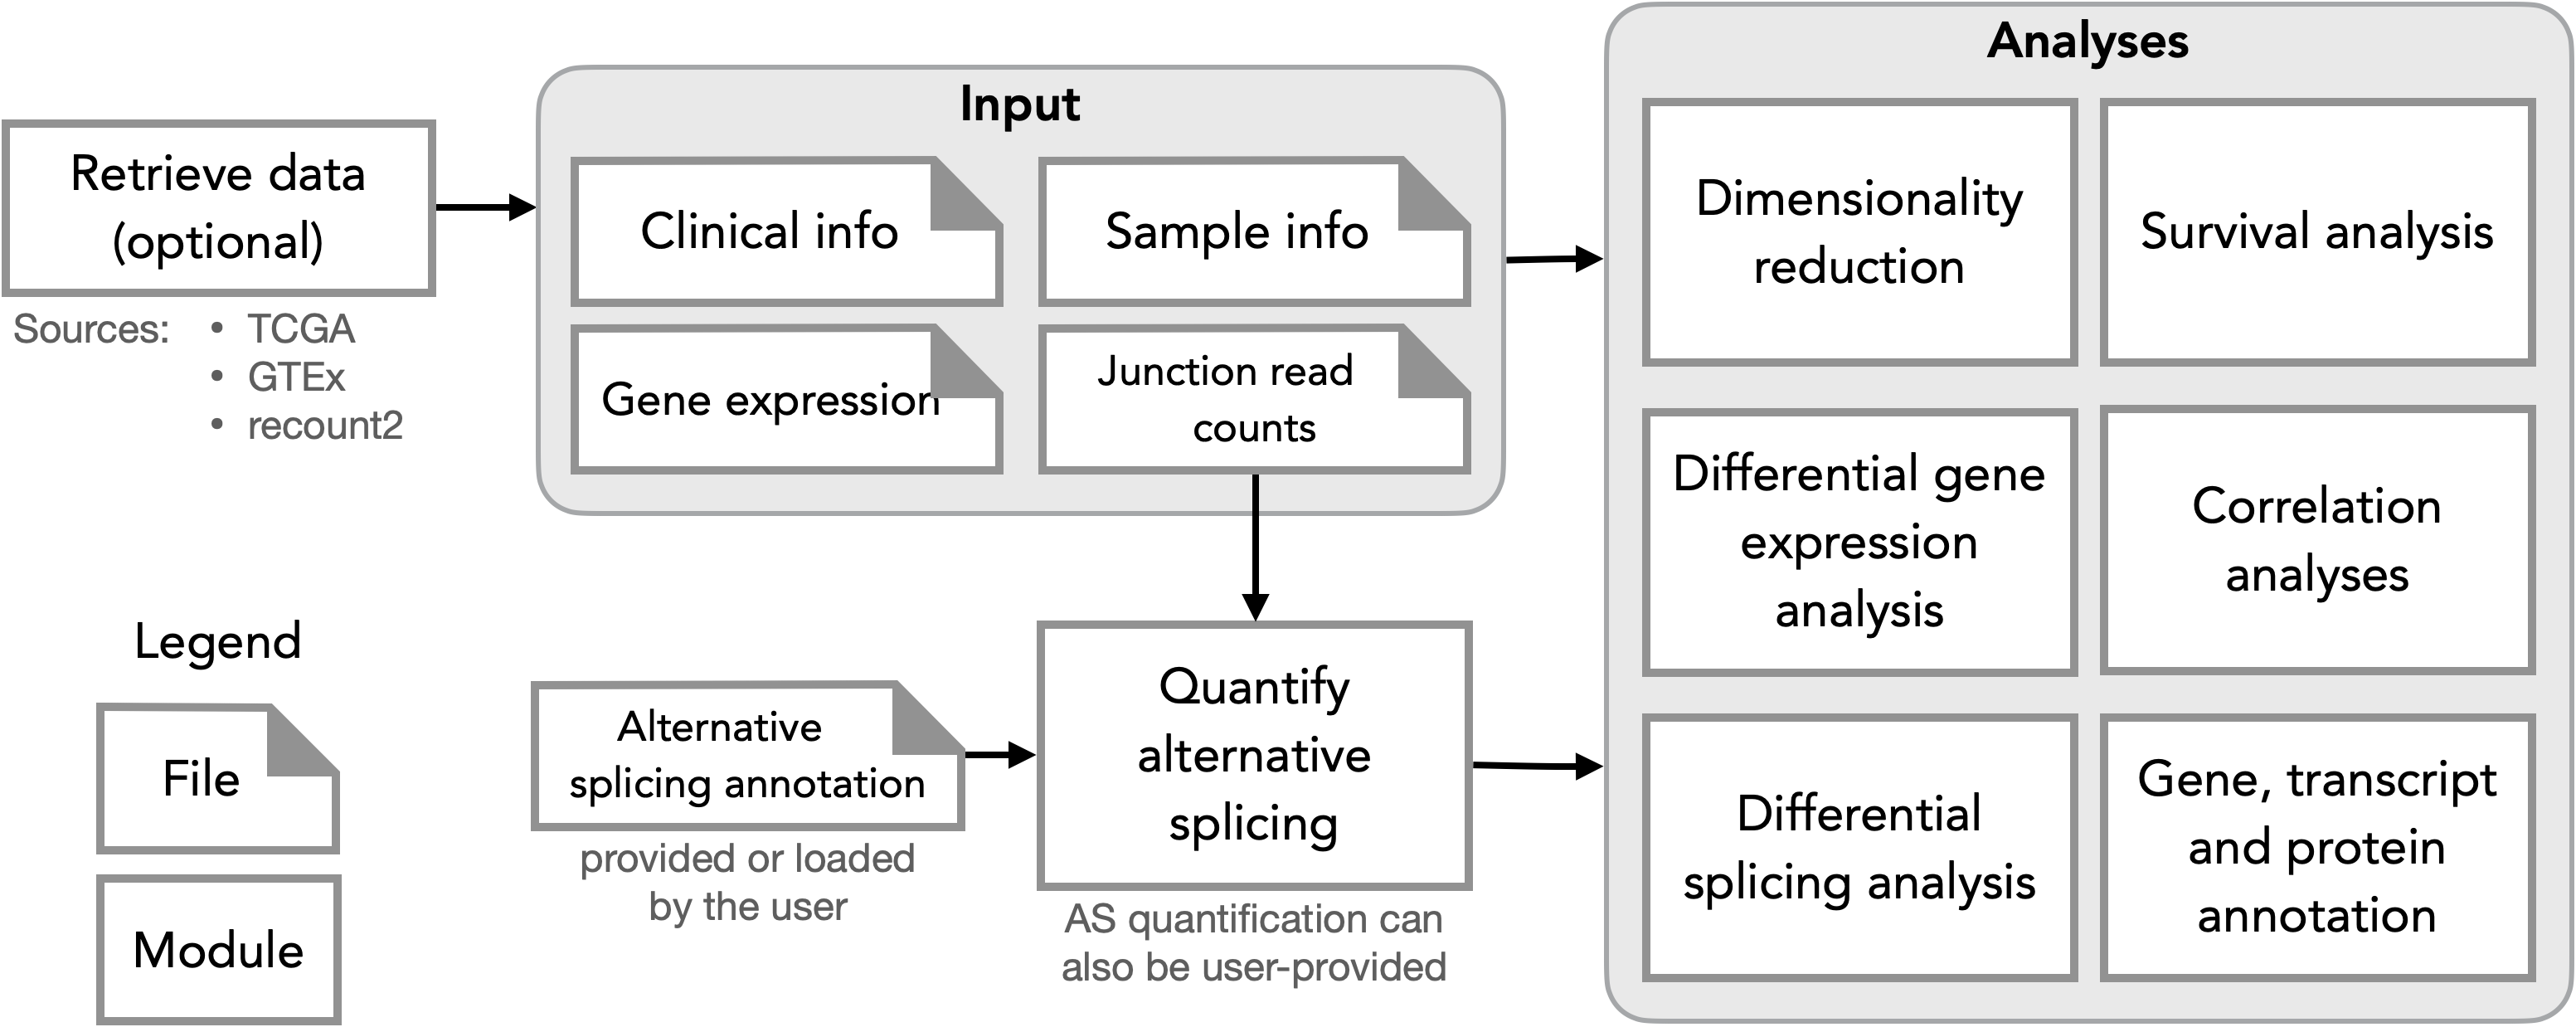
\includegraphics[width=.9\textwidth]{images/psichomics/workflow}
  \centering
  \caption[psichomics workflow]{\textbf{psichomics workflow.} The user can provide their own input data or load data from TCGA, GTEx or recount2 to normalise gene expression data and quantify alternative splicing for downstream analyses.}
  \label{fig:psichomics-workflow}
\end{figure}

The tool was designed as a modular R package to be easily modified and extended (\shortref{fig:psichomics-file-structure}), including modules for automatic data retrieval from multiple sources, parsing and standardisation of alternative splicing event identifiers from different programs and a variety of data analysis methodologies.

% TODO: add new symbol for a group of files to make it more intuitive to understand why there are multiple R files for the same data source
\begin{figure}[!ht]
  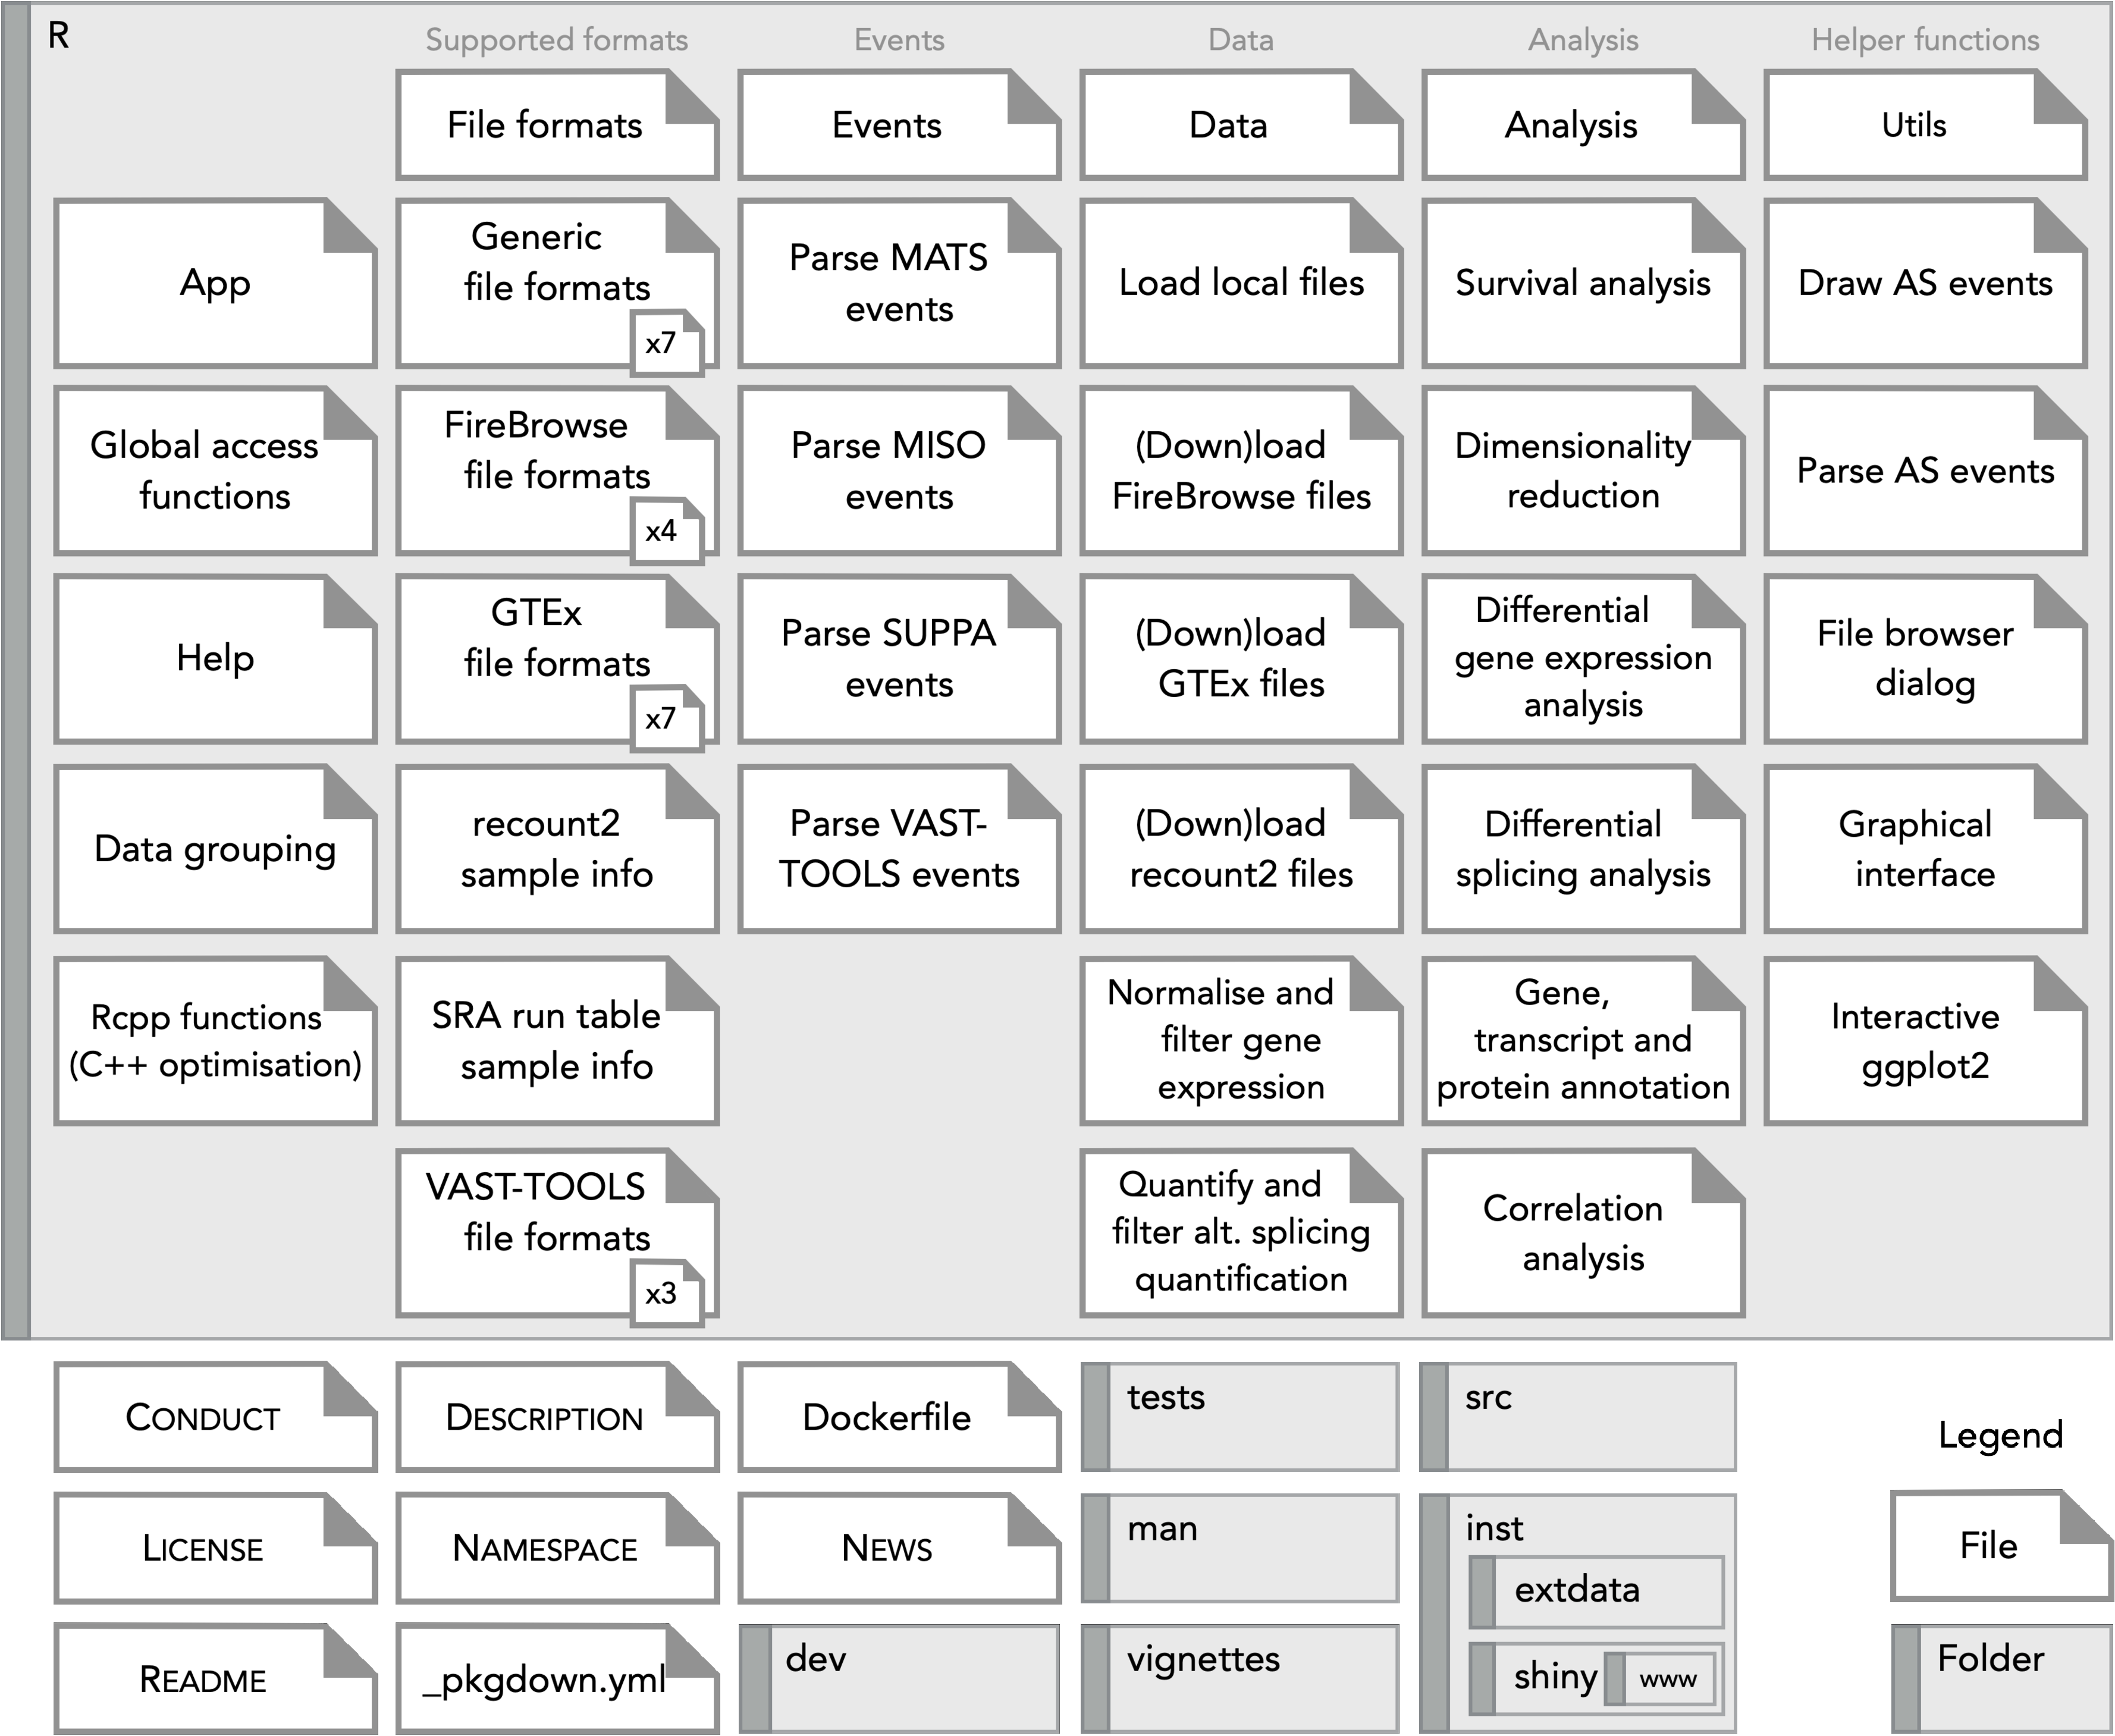
\includegraphics[width=1\textwidth]{images/psichomics/file-structure}
  \centering
  \caption[psichomics file structure]{\textbf{Visual representation of psichomics' file structure.} psichomics is a modular program where, for instance, functions specific for different data sources and analyses can be found in different files. As usual for R packages, the \texttt{R} folder is the heart of the code and contains the main R scripts that define the logic and interface of the app. \texttt{dev} is a non-standard folder in R packages used to store supporting scripts (e.g. test workflows); its contents are not included when building the R package.}
  \label{fig:psichomics-file-structure}
\end{figure}

To analyse alternative splicing, psichomics can load
 splice junction read count data provided by the user or from external sources, followed by the quantification of alternative splicing (in case no pre-computed quantification is loaded) and subsequent analyses. Alternative splicing quantification is computed based on RNA-seq reads that align to exon-exon junctions and the genomic coordinates (annotation) of alternative splicing events. The proportion of reads aligned to junctions that support the inclusion isoform, known as the Percent Spliced-In or PSI \cite{wang:2008wa}, was the chosen quantification metric.

\subsection{Data retrieval}

Exon-exon junction and gene expression quantifications (obtained from pre-processed RNA-seq data), clinical data and sample metadata are accessible through FireBrowse's web application program interface (API) for TCGA data retrieval (\alink{firebrowse.org/api-docs}). The FireBrowse API is used in psichomics to automatically download TCGA data according to the user-selected tumour type(s) as tab-delimited files within compressed folders, whose contents are subsequently loaded with minimal user interaction. GTEx data are automatically downloaded via the GTEx data portal (\alink{gtexportal.org}) and select SRA project data via recount2 \cite{collado-torres:2017uw}.

Other SRA projects and user-provided files may also be loaded in appropriate formats (\shortref{tab:psichomics-file-formats}), allowing for subsequent alternative splicing analysis, as explained in the tutorial available at \alink{nuno-agostinho.github.io/psichomics/articles/custom_data}).

\begin{table}[!ht]
\parnotereset
\small
\caption[Supported file formats in psichomics based on data source]{\textbf{Supported file formats in psichomics based on data source.}}
\label{tab:psichomics-file-formats}
\begin{tabularx}{\textwidth}{ l X X X X X }
\toprule
{\textbf{Source}} & {\textbf{Sample information}} & {\textbf{Subject information}} & {\textbf{Gene expression}} & {\textbf{Exon junction quantification}} & {\textbf{Alternative splicing quantification}} \\
\toprule
SRA Run Selector & Yes &     &     &     &     \\
\midrule
STAR             &     &     & Yes & Yes &     \\
\midrule
VAST-TOOLS       &     &     & Yes &     & Yes \\
\midrule
TCGA/FireBrowse  & Yes & Yes & Yes & Yes &     \\
\midrule
SRA/recount2     & Yes & Yes & Yes & Yes &    \\
\midrule
GTEx             & Yes & Yes & Yes & Yes &     \\
\midrule
Other files      & Yes & Yes & Yes & Yes & Limited\parnote{psichomics cannot fully parse alternative splicing events (e.g. it may not identify the cognate gene and coordinates) based on tables from these sources.} \\
\bottomrule
\end{tabularx}
\parnotes
\end{table}

\subsection{Gene expression pre-processing}

Gene expression quantifications can be filtered based on user-provided parameters (for instance, to account solely for genes supported by 10 or more reads in 10 or more samples, as performed by default) and normalised by raw library size scaling using function \texttt{calcNormFactors()} from R package \texttt{edgeR} \cite{robinson:2010wx}. Afterwards, counts per million reads (CPM) are computed and log\textsubscript{2}-transformed (if desired) using the function \texttt{cpm()} from \texttt{edgeR}. Log\textsubscript{2}-transformation is performed by default.

\subsection{Alternative splicing annotation}

Annotations of alternative splicing events are available on-demand in psichomics for 14 species (\shortref{tab:as-annot}). Human annotations were first available as a mix from multiple sources (as described in the following paragraphs). To support multiple species, annotations were created based on VAST-TOOLS 23.06.20 (including for human, thus the redundancy). Custom annotation files can also be created by following the appropriate tutorial available at \alink{nuno-agostinho.github.io/psichomics/articles/AS_events_preparation}.


\begin{table}[!ht]
\parnotereset
\small
\caption[Available alternative splicing annotations]{\textbf{Available alternative splicing annotations.}}
\label{tab:as-annot}
\begin{tabularx}{\textwidth}{ l l X }
\toprule
{\textbf{Species}} & {\textbf{Assembly}} & {\textbf{Source}} \\
\toprule

\multirow{2}{3cm}{\emph{Homo sapiens}} & \multirow{2}{3cm}{\emph{hg19 and hg38}} & VAST-TOOLS, SUPPA, MISO and rMATS \\
                                       &                     & VAST-TOOLS \\
\emph{Mus musculus}                    & mm9 and mm10        & VAST-TOOLS \\
\emph{Bos taurus}                      & bosTau6             & VAST-TOOLS \\
\emph{Gallus gallus}                   & galGal3 and galGal4 & VAST-TOOLS \\
\emph{Xenopus tropicalis}              & xenTro3             & VAST-TOOLS \\
\emph{Danio rerio}                     & danRer10            & VAST-TOOLS \\
\emph{Branchiostoma lanceolatum}       & braLan2             & VAST-TOOLS \\
\emph{Strongylocentrotus purpuratus}   & strPur4             & VAST-TOOLS \\
\emph{Drosophila melanogaster}         & dm6                 & VAST-TOOLS \\
\emph{Strigamia maritima}              & strMar1             & VAST-TOOLS \\
\emph{Caenorhabditis elegans}          & ce11                & VAST-TOOLS \\
\emph{Schmidtea mediterranea}          & schMed31            & VAST-TOOLS \\
\emph{Nematostella vectensis}          & nemVec1             & VAST-TOOLS \\
\emph{Arabidopsis thaliana}            & araTha10            & VAST-TOOLS \\
\bottomrule
\end{tabularx}
\parnotes
\end{table}

The hg19 annotation of human alternative splicing events was based on files used as input by MISO \cite{katz:2010tj}, VAST-TOOLS \cite{irimia:2014wt}, rMATS \cite{shen:2014tk} and SUPPA \cite{alamancos:2015vc}. Annotation files from MISO and VAST-TOOLS are provided in their respective websites, whereas rMATS and SUPPA identify alternative splicing events and generate such annotation files based on a given isoform-centered transcript annotation. As such, the human transcript annotation was retrieved from the UCSC Table Browser \cite{karolchik:2004wa} in GTF and TXT formats, so that gene identifiers in the GTF file (misleadingly identical to transcript identifiers) were replaced with proper ones from the TXT version.

The collected hg19 annotation files were non-redundantly merged according to the genomic coordinates and orientation of each alternative splicing event and contain the following event types: skipped exon (SE), mutually exclusive exons (MXE), alternative first exon (AFE), alternative last exon (ALE), alternative 5$'$ splice site (A5SS), alternative 3$'$ splice site (A3SS), alternative 5$'$ UTR length (A5UTR), alternative 3$'$ UTR length (A3UTR), and intron retention (IR). The resulting hg19 annotation is available as an R annotation package in Bioconductor at \alink{bioconductor.org/packages/alternativeSplicingEvents.hg19}, whereas the hg38 annotation (whose coordinates were converted from those of the hg19 annotation through function \texttt{liftOver()} from package \texttt{rtracklayer} \cite{lawrence:2009us}, based on the hg19 to hg38 chain file from UCSC) is also available as an R annotation package in Bioconductor at \alink{bioconductor.org/packages/alternativeSplicingEvents.hg38}.

\subsection{Alternative splicing quantification}

For each alternative splicing event in a given sample, its PSI value is estimated by the proportion of exon–exon junction read counts supporting the inclusion isoform therein \cite{wang:2008wa}. The junction reads required for alternative splicing quantification depend on the type of event (\shortref{fig:psichomics-calc-psi}). Alternative splicing events involving a sum of junction read counts supporting inclusion and exclusion of the alternative sequence below a user-defined threshold (10 by default) are discarded to avoid imprecise quantifications based on insufficient evidence.

\begin{figure}[!ht]
  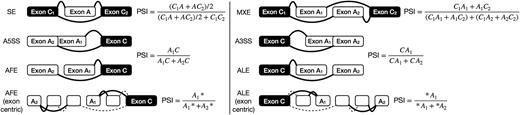
\includegraphics[width=1\textwidth]{images/psichomics/psi-quantification}
  \centering
  \caption[Alternative splicing quantification]{\textbf{Alternative splicing quantification.} Splice junctions required to quantify alternative splicing based on event type. C1A and AC2 represent read counts supporting junctions between a constitutive (C1 or C2, respectively) and an alternative (A) exon and therefore alternative exon A inclusion, while C1C2 represents read counts supporting the junction between the two constitutive exons and therefore alternative exon A exclusion. A1* and A2* represent the sum of read counts supporting junctions spanning the alternative first (A1) and second (A2) exon, respectively. Legend: skipped exon (SE), mutually exclusive exons (MXE), alternative 5$'$ splice site (A5SS), alternative 3$'$ splice site (A3SS), alternative first exon (AFE) and alternative last exon (ALE).}
  \label{fig:psichomics-calc-psi}
\end{figure}

Alternative splicing quantification in psichomics is currently based on exon-exon junction read counts, yet intron retention events require intron-exon junction read counts for their quantification \cite{braunschweig:2014tr}, whereas alternative 5$'$- and 3$'$-UTR require exon body read counts. psichomics does not currently quantify those types of alternative splicing events.

By default, psichomics quantifies all skipped exon events. However, the user can select to measure other types of alternative splicing events (\shortref{fig:psichomics-calc-psi}) and may hand in the list of genes whose alternative splicing events are to be specifically quantified. Furthermore, the step of alternative splicing quantification may be avoided if previously performed. psichomics allows the user to save the quantification of alternative splicing in a file to be loaded in a future session.

\subsection{Data grouping}

psichomics allows to group subjects and their samples or genes and their alternative splicing events for subsequent analysis. Subject and sample grouping can be performed based on available phenotypic (e.g. tissue type and histology) and clinical (e.g. disease stage, smoking history and ethnicity) features. Gene and splicing event grouping relies on respective user-provided identifiers. Moreover, the association between subject/sample groups specified by the user and those defined by the outcome of gene expression and alternative splicing analyses or by other clinical categorical variables can be statistically tested with Fisher's exact tests, implemented through function \texttt{fisher.test()} from \texttt{stats}.

\subsection{Dimensionality reduction}

Dimensionality reduction techniques can be performed on tables containing alternative splicing and gene expression quantifications, with the samples of interest as rows and the selected (if not all) splicing events or genes as columns, after centering and/or scaling the respective distributions (by default, they are only centered).

Principal component analysis (PCA) identifies the combinations of variables that contribute the most to data variance \cite{ringner:2008ve} and it is implemented through the singular value decomposition (SVD) algorithm provided by the \texttt{prcomp()} function from R package \texttt{stats}. The total contribution of each variable (splicing event or gene) towards data variance along selected principal components is measured based on the implementation of \texttt{fviz\_contrib} from \texttt{factoextra}.

Independent component analysis (ICA), a method used for decomposing data into statistically independent components \cite{hyvarinen:2000vk}, can also be performed through the \texttt{fastICA()} function from the eponymous R package, preceded by data centering and/or scaling with the \texttt{scale()} function.

As many of the aforementioned functions cannot handle missing data, a user-defined threshold for the accepted number of missing values per alternative splicing event or gene (5\%, by default) is used to discard variables before performing dimensionality reduction, whereas the remaining missing values are imputed for each variable as the median from non-missing data samples.

Moreover, samples can be clustered using k-means, partitioning around medoids (PAM) or clustering large applications (CLARA) methods, with the latter being optimised for large datasets and thus preferred by default. The implementation of these methods is based on the \texttt{kmeans()} function from \texttt{stats} and \texttt{pam()} and \texttt{clara()} functions from \texttt{cluster}, respectively.

\subsection{Survival analysis}

Kaplan-Meier estimators (and illustrating curves) \cite{rich:2010wt} and proportional hazard (PH) models \cite{spruance:2004vn} may be applied to groups of patients defined by the user based on clinical features derived, for instance, from TCGA and user-owned data, with survival distributions being compared using the log-rank test. Survival analyses are implemented in psichomics using functions \texttt{Surv()}, \texttt{survfit()}, \texttt{survdiff()} and \texttt{coxph()} from R package \texttt{survival} \cite{therneau:2000tk}.

To evaluate the prognostic value of a given alternative splicing event, survival analysis can be performed on groups of patients separated based on a given alternative splicing quantification (i.e. PSI) cut-off. Patients with multiple samples are assigned the average PSI value of their respective samples after sample filtering (e.g. when using TCGA data, only tumour samples are used for survival analysis by default). When survival differences are estimated for multiple PSI cut-offs for a single alternative splicing event, psichomics suggests the optimal cut-off that minimises the P-value of the log-rank test used to compare survival distributions, graphically supporting the suggestion with a PSI cut-off versus P-value scatter plot. Survival analysis can also be performed on groups defined by an expression cut-off for a selected gene.

\subsection{Differential splicing and gene expression analyses}

In psichomics, analysis of differential splicing between user-defined groups of samples can be performed on all or selected alternative splicing events. Given the non-normal distribution of PSI values \cite{kakaradov:2012wk,jia:2015wy}, median- and variance-based non-parametric tests, such as the Wilcoxon rank-sum (also known as Mann–Whitney U), Kruskal–Wallis rank-sum and Fligner–Killeen tests, are available and recommended \cite{barbaraCaravelaMScThesis}. Levene's and unpaired t-tests can nonetheless be performed as well. All these tests are available through the \texttt{stats} package with their default settings, except for Levene's test that was implemented based on the \texttt{leveneTest.default()} function from the \texttt{car} package.

To correct for multiple testing where applicable, P-value adjustment methods for the family-wise error rate (Bonferroni, Holm, Hochberg and Hommel corrections) and the false discovery rate (Benjamini–Hochberg and Benjamini–Yekutieli methods) are available through function \texttt{p.adjust()} from package \texttt{stats}. By default, multiple testing correction is performed using the Benjamini-Hochberg method.

Although the aforementioned statistical tests are also available to analyse the expression of single genes, genome-wide differential gene expression analysis is implemented based on gene-wise linear model fitting (using \texttt{lmFit} from R package \texttt{limma} \cite{ritchie:2015tm}) for two selected groups, followed by moderated t-tests and the calculation of log-odds of differential expression, using empirical Bayes moderation of standard errors (function \texttt{eBayes()} from \texttt{limma}) and gene-wise variance modelling (\texttt{limma-trend}).

Statistical results can be subsequently explored through density and volcano plots with customisable axes to assist in the identification of the most significant changes when analyzing distributions across single or multiple events, respectively. A corresponding table with the results of all statistical analyses is also available and can be retrieved as a tab-delimited plain text file.

\subsection{Correlation between gene expression and alternative splicing quantifications}

The Pearson product-moment correlation coefficient, Spearman's rho (default) and Kendall's tau, all available with \texttt{cor.test()} from \texttt{stats}, can be used to correlate gene expression levels with alternative splicing quantifications. Such analyses allow, for instance, to test the association between the expression levels of RNA-binding proteins (RBPs) and PSI levels of interesting splicing events to identify which of these may undergo RBP-mediated regulation. As such, a list of RBPs is provided in-app \cite{sebestyen:2016tr}, but the user can also define their own group of genes of interest for the test.

\subsection{Gene, transcript and protein annotation and literature support}

The representational state transfer (REST) web services provided by Ensembl \cite{yates:2015uo}, UniProt \cite{wu:2006vq}, the Proteins API \cite{nightingale:2017uq} and PubMed \cite{roberts:2001tg} are used in order to annotate genes of interest with relevant biomolecular information (e.g. genomic location, associated transcript isoforms and protein domains, etc.) and related research articles. psichomics also provides the direct link to the cognate entries of relevant external databases, namely Ensembl \cite{cunningham:2015wt}, GeneCards \cite{fishilevich:2016wh}, the Human Protein Atlas \cite{uhlen:2015tg}, the UCSC Genome Browser \cite{goldman:2015un}, UniProt \cite{wu:2006vq} and VAST-DB \cite{tapial:2017ui}.

\subsection{Performance benchmarking}

To measure the time taken by psichomics to load data, normalise gene expression, quantify PSIs for skipped exon events and perform global differential expression and splicing analyses between pairs of GTEx v7 tissues and between normal and primary solid tumour samples from multiple TCGA cohorts (data version 2016\_01\_28 from FireBrowse), the program was run 10 times with the same settings for different combinations of normal human tissues and tumour types in a machine running OS X 10.13.1 with 4 cores and 8GB of RAM, using Safari 11.0.1, RStudio Desktop 1.1.383 and R 3.4.1. The median duration of the 10 runs was used as the performance indicator.

To determine the approximate time complexity of the aforementioned steps in psichomics, gene expression and exon-exon junction quantification datasets were prepared based on approximate distributions obtained from the respective TCGA datasets: negative binomial distributions with a dispersion parameter of 0.25 and 0.2 reads and a mean parameter of 2000 and 100 reads for raw gene expression and exon-exon junction quantification, respectively. Each run was performed on datasets with numbers of samples ranging from 100 to 2500 in intervals of 100 (i.e. 100, 200, 300, …, 2500) and 20 000 genes or 200 000 splice junctions (gene expression or exon-exon junction quantification, respectively). Splice junction identifiers (required for alternative splicing quantification) were randomly retrieved from the TCGA reference annotation. Based on their respective read counts, around 9000 alternative splicing events (i.e. those for which all involved inclusion and exclusion junctions were retrieved) were quantified across selected samples per run. For differential gene expression and splicing analyses, samples were randomly divided into two groups based on the emitted values of a Bernoulli distribution with a probability of success of 50\%.

Polynomials of orders 1–6 were fitted to the relation between running time and the number of samples. As the running time is assumed to always increase with an increasing number of analysed samples, fitted polynomials were constrained to be monotone for 0 or more samples, using function \texttt{monpol()} from R package \texttt{MonoPoly} \cite{murray:2016um}. The best polynomial fits (\shortref{fig:psichomics-performance}) were selected based on analyses of variance (ANOVA) between fitted polynomials of consecutive orders, starting with the comparison between polynomials of orders 1 and 2. A polynomial with higher order is only selected if exhibiting a significantly better fit (p-value $< 0.05$).

\subsection{Alternative splicing quantification benchmarking}

The publicly available RNA-seq data from multiple human, mouse and chicken tissue and cell line samples used in the development of VastDB \cite{tapial:2017ui} were aligned with splice-aware STAR \cite{dobin:2013ts} against the respective transcript-annotated genomes: UCSC hg19 genome assembly and GENCODE v19 annotation for human, UCSC mm10 genome assembly and GENCODE vM14 annotation for mouse, and Ensembl 70 genome assembly and annotation for chicken. In total, 120/706/34 (human/mouse/chicken) exon skipping events quantified by psichomics (using function \texttt{quantifySplicing()} with default settings) were compared with the respective RT-PCR- and VAST-TOOLS-derived PSI values, available from VastDB \cite{tapial:2017ui}.

Different numbers of junction reads were simulated for different given PSI values to test the impact of read coverage on the accuracy and precision of PSI estimation by psichomics. For each given PSI, junction reads supporting the exon inclusion were simulated as the number of successes obtained from a Bernoulli distribution with the event's junction read coverage (i.e. reads supporting inclusion plus reads supporting exclusion) as the number of observations and the PSI value as the probability of success. Those inclusion reads were then divided by the event's junction read coverage to estimate an ‘observed’ PSI value (as performed by psichomics) that was compared to the given ‘real’ PSI value. These simulations were performed for PSI values from 0 to 1 in 0.1 intervals and event coverages of 10, 20, 50, 100, 500 and 1000 junction read counts, with each combination being tested 10000 times.

TCGASpliceSeq \cite{ryan:2016tm} provides pre-computed alternative splicing quantifications across TCGA cohorts. As those quantifications are performed similarly by TCGASpliceSeq and psichomics, PSI estimates for each matching (based on genomic coordinates) alternative splicing event and sample from both tools were correlated across the entire TCGA dataset.

\subsection{Continuous integration}
\label{subsec:psichomics-ci}

Continuous integration (CI) tools ensure the automatic testing of software in multiple environments (different versions of operating systems, R, BioConductor, etc.). Currently popular CI tools include Travis CI (macOS and Linux, limited support for Windows), AppVeyor (Windows only) and GitHub Actions (Windows, macOS and Linux). Although psichomics was initially set up with Travis CI and AppVeyor, the flexibility of GitHub Actions in running the three main operating systems and the easiness of adding complex routines led me to replace Travis CI and AppVeyor with GitHub Actions.

psichomics has three GitHub Actions scripts. The first one creates Docker images and stores them in GitHub and Docker Hub for every psichomics release or change in the dev branch. The second one updates the package documentation website via \texttt{roxygen} and \texttt{pkgdown}. The last one builds and checks the R package using \texttt{rcmdcheck::rcmdcheck()} and \texttt{BiocCheck::BiocCheck()} for every change that is committed to the GitHub repository. psichomics is tested in Windows, macOS and Ubuntu, allowing to automatically check if the package builds correctly and if it passes all unit tests (created using testthat) in multiple platforms, among other checks. The code coverage of the package is then tested via Codecov. All of these tools are free for open-source projects.

\section{Results}

The graphical interface of psichomics is available at \alink{compbio.imm.medicina.ulisboa.pt/psichomics}. Alternatively, users can install psichomics in their own computers, allowing to use local computing resources. psichomics offers both a graphical and a command-line interface. Although most features are common to both interfaces, we recommend less experienced users to opt for the Shiny-based graphical interface. To start the graphical interface in the local version, load the psichomics package in R via \texttt{library(psichomics)} and run \texttt{psichomics()}. The user's default web browser will be launched with a local version of the psichomics web app.

\subsection{Case study}

\subsection{Time benchmarking}

The times required to load, quantify and analyse data from different TCGA (data version \texttt{2016\_01\_28} from FireBrowse) and GTEx v7 cohorts were benchmarked. The breast cancer cohort contains the highest number of RNA-seq samples available in TCGA, thus being that for which it takes more time to load, quantify and analyse alternative splicing and gene expression data. Contrastingly, processed data from GTEx come bundled in files containing all tissues. Although only data from specified tissues are loaded, scanning though the large GTEx file still delays data loading. Tissues from GTEx were loaded in pairs for subsequent differential splicing analyses (\shortref[A]{fig:psichomics-performance}).

\begin{figure}[!ht]
  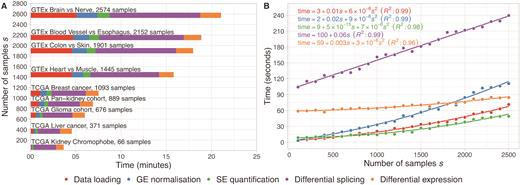
\includegraphics[width=1\textwidth]{images/psichomics/performance-benchmark}
  \centering
  \caption[Performance benchmark for alternative splicing analysis]{\textbf{Performance benchmark for alternative splicing analysis using RNA-seq data from multiple TCGA and GTEx sample types.} (A) Median times of 10 runs of data loading, gene expression (GE) normalisation, skipped exon (SE) event quantification and differential expression and splicing analysis (normal versus tumour for TCGA data or pairwise tissue comparison for GTEx data) using psichomics. The default settings were used during the runs. (B) Estimation of the time complexity of each of the aforementioned steps in psichomics. Randomly generated synthetic datasets of different sample size s were used as input. Equations and coefficient of determination ($R^2$) for the best fits are displayed.}
  \label{fig:psichomics-performance}
\end{figure}

Synthetic datasets for gene expression and exon-exon junction quantification of multiple sample sizes were generated, based on TCGA data distributions, to determine the time complexity of each step in psichomics as a function of the number of input samples $s$ (\shortref[B]{fig:psichomics-performance}). Assuming a constant number of genes (20 000 in the benchmark) or exon-exon junctions (200 000), the time taken to load data grows quadratically with $s$. Gene expression normalisation and differential expression are based on commonly-used, time-efficient bioinformatics tools and the times taken for each also grow quadratically with $s$. Alternative splicing quantification is associated with element-wise operations on matrices of dimensions $s$ by the number of alternative splicing events and takes a runtime approximately proportional to the square of $s$, for a given number of alternative splicing events (around 9000 for each benchmarked run). Finally, differential splicing is based on multiple, distinct statistical analyses of alternative splicing quantification data and grows linearly with $s$.

\subsection{Alternative splicing quantification benchmarking}

Although jSplice's \cite{christinat:2016ui} and DIEGO’s \cite{doose:2018uv} splicing quantifications rely on junction read counts, their alternative splicing module expression and junction usage metrics, respectively, are not directly comparable with psichomics’ PSI values. To evaluate their accuracy in the absence of any known tool with the same input (junction read counts) and output metric (PSI) as psichomics, psichomics-estimated PSI values were compared to those estimated by RT-PCR and using VAST-TOOLS \cite{irimia:2014wt} across multiple tissue and cell line samples from human, mouse and chicken \cite{tapial:2017ui}. VAST-TOOLS follows an analogous, and therefore more directly comparable, procedure for computing PSI values and there is a substantial overlap between the alternative splicing event annotations used by the two tools. psichomics estimates highly correlate with both others, particularly for mouse and human (Supplementary Figure S7), suggesting robustness and reproducibility in alternative splicing quantification by psichomics. Of note, the lower correlation for chicken samples is attributable to a single outlier, as its removal increases the correlation coefficients between psichomics and RT-PCR estimates (Pearson's r = 0.87, p-value $< 0.01$; Spearman's rho = 0.87, p-value $< 0.01$) and psichomics and VAST-TOOLS estimates (Pearson's r = 0.93, p-value $< 0.01$; Spearman's rho = 0.94, p-value $< 0.01$).

To assess the influence of RNA-seq read coverage on psichomics PSI estimates, different numbers of junction reads per event were simulated for different given PSI values (10000 times for each combination). Supplementary Figure S8 shows that the accuracy of PSI estimation by psichomics is expectedly sensitive to junction read coverage, particularly for intermediate PSI values, with 90\% prediction intervals $<0.1$ for coverage higher than a few hundred reads.

Alternative splicing events annotated by TCGASpliceSeq \cite{ryan:2016tm}, an online tool that displays pre-computed PSI values across multiple TCGA tumour types, were matched to those from psichomics based on their genomic coordinates. In total, 321 183 of 757 749 (42\%) skipped exon, 70 837 of 126 725 (56\%) alternative 5$'$ splice site and 90 940 of 155 799 (58\%) alternative 3$'$ splice site events were successfully matched. When available from both programs, PSI estimates for each of the 482 960 alternative splicing events in each of the 9 913 matched samples were compared between TCGASpliceSeq and psichomics, being highly correlated (N = 92 444 302; Pearson's r = 0.97, p-value $< 10^{15}$; Spearman's rho = 0.94, p-value $< 10^{15}$; Supplementary Figure S9).

\subsection{Impact}
\label{sec:impact}

There are multiple ways to measure the impact of psichomics. First, we can check the metrics surrounding the article itself. 

% importance of maintaining software and replying to user feedback

- Invitation to write a book chapter

Although there is no direct way to measure user engagement with psichomics, we can track:

- Bioconductor downloads

- Docker Hub image downloads 

- visitors to the official psichomics documentation

- visitors to the website

- feedback via GitHub issues and emails

- citations

%It is wonderful to see that the work I put into psichomics is appreciated based on feedback received via GitHub and email. psichomics is still used nowadays based on citations from recent published articles (Ling et al., 2020; Baeza-Centurion et al., 2020; Birladeanu et al., 2021). In the lab, we can also track visitors of psichomics’ documentation via Google Analytics to better understand our users (e.g., what pages they visit the most).

\section{Conclusion}

Alternative splicing is a regulated molecular mechanism involved in multiple cellular processes and its dysregulation has been associated with diverse pathologies \cite{kelemen:2013tc,paronetto:2016vw,wang:2008wa,oltean:2014vm}. The advent of next-generation sequencing technologies has allowed the investigation of transcriptomes of human biological samples to be expanded to alternative splicing. RNA-seq data, like those yielded by the GTEx and TCGA projects, are indeed playing crucial role in the improvement of our insights into the role of alternative splicing in both physiological and pathological contexts \cite{paronetto:2016vw,wang:2008wa,gallego-paez:2017wc,tsai:2015ve,danan-gotthold:2015ut}).

However, the most commonly used tools for alternative splicing analyses currently do not allow researchers to fully benefit from the wealth of pre-processed RNA-seq data made publicly available by the aforementioned projects. For instance, they lack support for estimating PSIs based on splice junction read counts. Such functionality would allow users to overcome the difficulties caused by the raw RNA-seq data from GTEx and TCGA being under controlled access and, more importantly, their processing requiring computational resources inaccessible to the majority of research labs. psichomics thus exploits pre-processed alternative splicing annotation and exon–exon junction read count data from TCGA and GTEx, two of the richest sources of molecular information on human tissues in physiological and pathological conditions, as well as recount2 and user-owned data, allowing researchers to hasten alternative splicing quantification and subsequent analyses by avoiding the time-consuming alignment of RNA-seq data to a genome or transcriptome of reference followed by splice junction detection.

Together with support for the integration of molecular and sample-associated clinical information, the group creation functionalities featured in psichomics ensure full customisability of data grouping for downstream analyses. Interesting groups to compare in TCGA, for instance, may range from the simple contrast between reformed and current smokers in lung cancer to complex combinations of gender, race, age, country and other subject attributes across multiple cancers. When survival data are available, survival analyses can be performed on samples by PSI or gene expression levels, thereby assessing the putative prognostic value of a respective molecular feature.

The integrative analysis of publicly available TCGA data by psichomics allowed us to identify multiple exons differentially spliced between breast tumour stage I and normal samples, therefore deeming them potential diagnostic biomarkers, and to assess their putative prognostic value. The output of psichomics is validated by identified alternative splicing alterations that have been previously linked to the disease, including events in RPS24, NUMB, FBLN2 and AP2B1. Previously understudied, yet intriguing, events were also identified, such as the skipping of SLMAP exon 23 and UHRF2 exon 10. These may provide novel insights into the early stages of breast cancer development. Indeed, it is of utmost importance to foster alternative splicing analyses of clinical samples as a crucial complement to more conventional research focused on total gene expression.

To ensure researchers with different skills can take the most out of psichomics, users lacking a computational background may feel more comfortable using the intuitive and more accessible graphical interface, whereas advanced users may opt for the command-line view. Should the demanding computational resources for hosting psichomics in a web server become available, we also envisage its web deployment, so that the program's latest version is publicly available on-demand with no installation required, levering the intuitive graphical interface to make alternative splicing analyses more enticing to less computationally-inclined biomedical researchers.

Notwithstanding its merits, psichomics only quantifies alternative splicing events based on exon–exon junction read counts, limiting the types of alternative splicing events profiled. For instance, exon–intron junction, exon body and intron body quantifications are vital to confirm intron retention and alternative 5$'$ and 3$'$ UTR events over further transcriptional variations \cite{braunschweig:2014tr}.
However, although GTEx (but neither TCGA nor recount2) readily provides intron and exon body read quantification for retrieval, none provides exon–intron junction quantification. To overcome this, psichomics allows to import alternative splicing events quantified from other programs, including VAST-TOOLS that quantifies intron retention events.

Another limitation is psichomics reliance on existing alternative splicing event annotations and an on the pre-processing of RNA-seq data by third-party pipelines (as is the case for GTEx, TCGA and recount2), depriving the user of the flexibility to identify de novo alternative splicing events. However, as we detail in \alink{nuno-agostinho.github.io/psichomics/articles/AS_events_preparation}, when FASTQ or BAM files are accessible, psichomics supports the loading of alternative splicing annotations generated by different programs that take those files as input, namely rMATS \cite{shen:2014tk}, which is able to generate de novo annotations.

Using psichomics, we are able not only to identify novel exons differentially spliced between tumour stage I and normal breast samples but also to pinpoint potentially clinically relevant splicing events by embracing clinical data and evaluating their prognostic value. We expect that fellow researchers and clinicians will be able to intuitively employ psichomics to assist them in uncovering novel splicing-associated prognostic factors and therapeutic targets, as well as in advancing our understanding of how alternative splicing is regulated in physiological and disease contexts.

% For future iterations of psichomics, Potentially useful recount3?